\chapter{Formalising ZKBoo}
\label{ch:formal_zkboo}
In this chapter, we formalise the ZKBoo protocol along with the security proofs by
\citet{zkboo}. To formalise this, we utilise our formalisations of
$\Sigma$-Protocols and commitment schemes. ZKBoo is a $\Sigma$-Protocol, so we
use our formalisation to instantiate this. We then use our formalisation of commitment
schemes to prove the security definitions for ZKBoo.
The definitions and proofs formalised in the chapter all come from
\citet{zkboo}, but to formalise these, we have had to make significant changes to
the definitions and prove certain predicates about the different procedures of
the protocol to prove it secure. These changes have been necessary since crucial
assumptions have been kept implicit in the original paper.
By formalising the proofs of security, we make these assumptions explicit
which can help improve implementation-level security by exposing edge-cases
where the security definitions could break down.

The goal of formalising ZKBoo is two-fold. First, we show that our previous
formalisations are indeed applicable to more extensive protocols. Second, we aim to
gather insight into the security of the ZKBoo protocol itself, and how formal
verification can help us find pitfalls in informal proofs.

To formalise the work of ZKBoo, we first start by developing a formalisation of
arithmetic circuits within \easycrypt. This formalisation allows us the reason about
evaluating circuits to a value while also enabling us to reason about the
structure of arithmetic circuits.
Next, in section \ref{sec:decomposition} we formalise the
(2,3)-Decomposition of arithmetic circuits as defined in section
\ref{sec:arith_circuits}.
Ultimately, we use the formalisation of arithmetic circuits and their
(2,3)-Decomposition to instantiate ZKBoo as a $\Sigma$-Protocol and then prove
it secure.


\begin{figure}[ht]
  \centering
  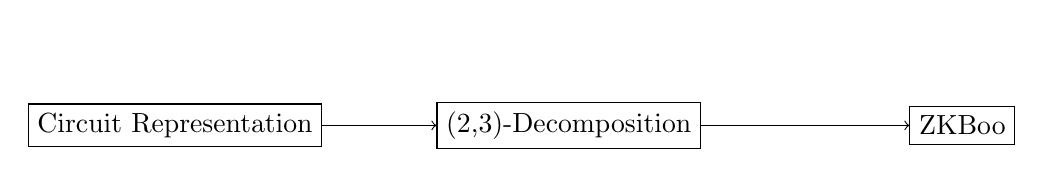
\begin{tikzpicture}
      \node[draw] at (-20,.3) (a) {Circuit Representation};
      \node[draw] at (-15,.3) (b) {(2,3)-Decomposition};
      \node[draw] at (-10,.3) (c) {ZKBoo};

      % draw edges
      \draw[->] (a) -- node[midway,above,yshift=1cm] {} (b);
      \draw[->] (b) -- node[midway,above] {} (c);
  \end{tikzpicture}
  \caption{\label{fig:outline_zkboo} Outline of ZKBoo formalisation}
\end{figure}

\paragraph{Preliminary notation}
Throughout this chapter, use the letter $e$ to denote a challenge expressed as an integer in \{1,2,3\}.
Moreover, we define arithmetic on challenges such that $3+1 = 1$.

\section{Formalising Arithmetic circuits}
\label{sec:arith_circuits}
Before we can reason about the decomposition of an arithmetic circuit, we need a
definition of what an arithmetic circuit is, and how we can compute values from it.
To this end, we introduce the concept of arithmetic circuits and how they
can be represented.
Primarily we recall the definition of circuits as
a graph which is also used in the original paper by \citet{zkboo} and discuss how
to evaluate circuits programmatically.
Lastly, we introduce an alternative representation of arithmetic
circuits and provide several definitions, enabling us to reason
about the structure of the circuit and its evaluation.

\subsection{Representing an arithmetic circuit}
\label{subsec:arith-representation}
An arithmetic circuit in its most general form express a function $f$ over some
arbitrary finite field $\mathbb{Z}_{q}$, where $f : \mathbb{Z}_{q}^{k} \rightarrow \mathbb{Z}_{q}^{l}$

To express arbitrary (arithmetic) computations in a finite field we
use the following four gates, addition by constant (ADDC), multiplication by constant
(MULTC), addition of two wires (ADD), and multiplication of two wires (MULT).

The goal of this section is to formulate a representation of the function
$f$, which only depends on the aforementioned gate types to perform
computations. Before doing so, however, we start by stating several
simplifying assumptions about our arithmetic circuits. First, we only allow the
circuit to have one input value and one output value, in other words:
$k = l = 1$ in the definition of $f$.
This assumption exists to simplify reasoning about the inputs and
outputs of the function, while still capturing the essence of the original
relation. We argue that this simplification is still equally as expressive as
the non-simplified representation. The reason for this is that \easycrypt\
allows for tuple types, which can encode multiple inputs into the single input
gate. Thus we can still turn the single input circuit into a multi-input circuit
under this restriction.
% The results obtain in this section could be altered to
% allow for arbitrary inputs with minor alterations, but we will not go into more
% details o

Based on these simplifying assumptions we can now recall the graph
representation of a circuit:
\begin{definition}[Arithmetic Circuit]
  \label{def:arith_circuit}
  An Arithmetic circuit is a directed graph C = (W, G) where W is the internal
  wires between the gates and G is the set of gates within the circuit. Then,
  we let $in \in G$ be the first gate of the circuit, i.e. the input and $o \in G$ be the final
  gate of the circuit, for which there must exist a path from in to o in W.
  Specifically, o is a gate with only in-going wires and no out-going wire.
  The value of the circuit is then obtained by computed the value of $o$.

  Finally, for all gates $g \in G$ there must exist a path in W from in to o going
  through g.
  If this was not the case, then the gate could be removed from the graph without changing the
  semantic meaning of the circuit.
\end{definition}

To define the evaluation of the circuit, we would then need to compute the value of the
in-going wires of o, but this requires all other wires in the circuit to be
computed first.
Consequently, the value of the out-going wires of a given gate can only
be computed if all in-going wires of the gate have already been assigned to a
value.
It is clear from this that we need to define an evaluation order for the
circuit, such that we only try to compute the value of a gate if we know that
all in-going wires have been assigned a value.

To define the order of evaluation, we follow the work of \cite{Yao} and introducing an alternative
representation of Arithmetic circuits, which naturally gives us a well-defined
evaluation order:

\begin{definition}[List representation of arithmetic circuits]
  Given an arithmetic circuit C as defined by definition \ref{def:arith_circuit}
  we define the list representation of C by computing a linear ordering, O, of
  G, which gives each gate in G a unique index.
  We then let the list representation $C_{L}$ be defined as:
  \[
    C_{L}[j] = Enc(O( G \setminus \{in\})[j], W)
  \]

  Where $Enc : gate \rightarrow W \rightarrow \text{encoded gate}$, is a function
  taking as input a gate and the wires of the circuit and produces an encoded
  gate.
  Encoded gates contain type information about gate but also stores the
  indexes (From the linear ordering) of the gates, whose out-going wires are the
  in-going wires of the gate. \eg. If we have an addition gate with wires coming
  from the gate with index $i$ and a gate with index $j$ we express this as an
  encoded gate $MULT (i, j)$.
  The type declaration of the encoded gates can be seen in figure \ref{lst:gate_types}.
\end{definition}

\begin{figure}[ht]
  \centering
  \begin{subfigure}{ 0.48\textwidth }
  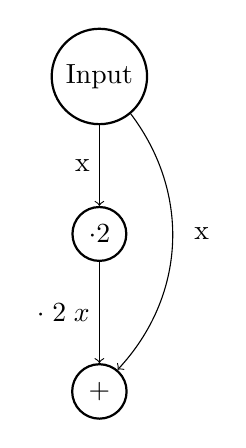
\begin{tikzpicture}[scale=1]
      \node[circle, thick, draw=black, minimum size=3pt] at (0,0) (c1) {Input};
      \node[circle, thick, draw=black, minimum size=3pt] at (0,-2) (c2) {$\cdot 2$};
      \node[circle, thick, draw=black, minimum size=3pt] at (0,-4) (c3) {$+$};
      \draw[->] (c1) -- (c2) node [midway, left] {x};
      \draw[->] (c2) -- (c3) node [midway, left] {$\cdot \; 2 \; x$};
      \draw[->] (c1) to[bend left=40] (c3);
      \node at (1.3, -2) {x};
  \end{tikzpicture}
  \caption{Graph representation of circuit}
  \end{subfigure}
  \hfill
  \begin{subfigure}{ 0.48\textwidth }
  \begin{tikzpicture}[scale=1]
\matrix (m) [matrix of nodes,
             nodes={draw, minimum size=14mm,anchor=center},
             nodes in empty cells, minimum height = 1cm,
             row 1/.style={nodes={draw=none}},
             row 3/.style={nodes={draw=none}},]
{
  1 & 2 \\
  $(\cdot 2)$ 0 & $(+)$ 0 1 \\
  0 & 1 & 2 \\
  x & $(\cdot \; 2 \; x)$ & $(+ \; x \; (\cdot \; 2 \; x))$ \\
};
\node at (1.0,0.7) {$= C_{L}$};
\node at (3.2,-2.1) {$= \text{state}$};
\end{tikzpicture}
  \caption{List representation of circuit}
  \end{subfigure}
\end{figure}

\paragraph{Linear ordering}
A linear ordering O is a function that when applied to G assigns a unique
index to each gate in G.
One example of such a linear ordering is the breadth-first
search (BFS) of a graph.
Here each gate in the circuit graph is labelled according to the time at which
the BFS visited the gate/node.

This labelling would start at the input gate and end at the output gate.

A particular property of the linear ordering induced by a BFS ordering is that a
gate can only be visited if all nodes with wires to that gate have already been
visited by the BFS.
This ordering ensures that for any node with index $i$ only
depends on out-going wires of nodes with index less-than $i$.

This ordering allows us to convert the graph representation into a list
representation, where the gate at index $i$ is the node with index $i$ by the
linear ordering. However, since the input gate performs no computation and only
exists to add the input value to the graph we exclude it from the list
representation, and shift every index one down.

\paragraph{Encoded gates}
A gate is a type, where the type defines the operation the gate computes along
with a tuple $(l,r)$ where $l$ is the index node corresponding to the left input
wire and $r$ is for the right input wire.
In the case of unary gates like ADDC and MULTC
the tuple is $(c, l)$ where l is the input wire, and $c$ is the constant used in
the computation.

But we need to encode W into this list. To do this, we encode the information
about input wires into the types of the gates themselves, as seen in figure
\ref{lst:gate_types}.

\begin{lstlisting}[float,label=lst:gate_types,caption=Type declaration of gates]
type encoded_gate = [
  | ADDC of (int * int)
  | MULTC of (int * int)
  | MULT of (int * int)
  | ADD of (int * int)
].
\end{lstlisting}
\vspace{2mm}
\noindent
One important aspect of the list representation of circuits is that it allows
us to define an evaluation order, which ensures that we are not trying to
computing the value of a gate before the all its inputs wires has been assigned
a value. To capture this notion of a valid evaluation order we give the following definition:

\begin{definition}[Valid circuit]
  \label{def:decomp:valid_circuit}
  An arithmetic circuit in list representation $C_{L}$ is valid if for every
  entry $i$ in the list it holds that:
    \begin{itemize}
      \item C[i] is a gate type
      \item the gate corresponding to the input wires of C[i] have index $j$ where $0 \geq j<i$.
    \end{itemize}
\end{definition}

\begin{lstlisting}[float,label=lst:circuit_eval,caption=Circuit evaluation function]
op eval_gate (g : gate, s : state) : int =
  with g = MULT inputs => let (i, j) = inputs in
                          let x = s[i] in
                          let y = s[j] in x * y
  with g = ADD inputs =>  let (i, j) = inputs in
                          let x = s[i] in
                          let y = s[j] in x + y
  with g = ADDC inputs => let (i, c) = inputs in
                          let x = s[i] in x + c
  with g = MULTC inputs => let (i, c) = inputs in
                           let x = s[i] in x * c.

op eval_circuit_aux(c : circuit, s : int list) : int list =
    with c = [] => s
    with c = g :: gs =>
     let r = eval_gate g s in
     eval_circuit_aux gs (rcons s r).

op eval_circuit (c : circuit, s : state) : output =
    last (eval_circuit_aux c s).
\end{lstlisting}

It is then possible to define the semantic meaning of list representation of circuits by
defining the evaluation function, which can be seen in figure \ref{lst:circuit_eval}.
The evaluation is broken into two parts: First, we have a function for evaluating
one gate to an intermediate value. Second, we have a procedure for evaluating
the entire circuits which call the former.
To evaluate a single gate, we first need to determine the type of the gate. This can
be done by utilizing the power of the \easycrypt\ type system, which allows us
to pattern match on the type of the gate as seen in listing \ref{lst:circuit_eval}.

Then, by the validity of the circuit, we know that if computing index $i$ of the
circuit, then indices $[0 \dots i-1]$ have already been computed.
Performing the computation expressed by the gate then reduces to looking up the
values of the previously computed gates and applying them to the function
appropriate for the type of the gate.

Computing the entire circuit in then correct by the correctness of computing a
single gate, and that we evaluate the circuit in order from lowest to highest index.

By continually performing gate evaluation of the next entry in the list and saving the result
into in a list called ``state'' at the appropriate index.
Then when computing the gate $MULT(i,j)$, we simply look up the valued of index
$i$ and $j$ in ``state'' and multiply them together.
When every single gate of the circuit has then been computed and saved in
``state'', then the output of the circuit will be in the last entry of
the state.

\begin{definition}[State of list representation]
  For a list representation of a circuit $C_{L}$ we give the following recursive
  definition of the state:
  \begin{align*}
    \text{state}[0] &= \text{input value} \\
    \text{state}[i>0] &= \texttt{eval\_{gate} } C_{L}[i-1] \; state[i-1]
  \end{align*}

  Here we recall that input gate has been removed from the list representation
  and $C_{L}$[0] is the first non-input gate in the circuit. From this it also
  follows that
  \begin{equation}
    \text{size } \text{state} = \text{size } C_{L} + 1
  \end{equation}
\end{definition}

We then have that any valid circuit c can be compute to a value y as
\texttt{eval\_circuit(c, [input]) = y}. This can also be stated as a probabilistic
procedure as $\Pr{\texttt{eval\_circuit(c, [input])} = y} = 1$.

To reason about functions and procedures based on the same function we have the following lemma:
\begin{lemma}[Function/Procedure relation]
  \label{lem:func/proc-equiv}
  $\forall$ f, inputs, output: f(inputs) = output $\iff \Pr{f(inputs) = output} = 1$.
\end{lemma}
\begin{proof}
  \hspace{2mm}
  \begin{itemize}
    \item  ``$\Rightarrow$'': trivial
    \item  ``$\Leftarrow$'':
      We split the prove into two parts:

      \noindent $output = f(inputs)$: trivial.

      \noindent $output \neq f(inputs)$: Here we prove that
      \[
        output \neq f(inputs) \implies \Pr{f(inputs) = output} = 0.
      \]
      Which is trivially true. We then use this to derive a contradiction in our
      assumptions, thus completing the proof.
  \end{itemize}
\end{proof}


\section{(2,3) Decomposition of circuits}
\label{sec:decomposition}
In this section we give a formalisation of the (2,3)-Decomposition of arithmetic
circuits based on the description given in section \ref{subsec:general:arith}.

In the most general form, we can define the decomposition as a procedure taking
as input three views and random tapes, and a circuit and produce three new
views, where a view is a list of shares.
More specifically, the decomposition work by incrementally evaluating a gate based on
previously computes views, which yield new shares that can be appended to the
view. We then repeat the process of evaluating a single gate based on the view of evaluating
the previous gate until all gates have been computed. This
overall idea has been captured in the procedure in figure \ref{lst:decomp_aux},
which mimics the Update function from section \ref{subsec:general:arith}.
The arithmetic decomposition, however, requires that we can split the witness into
three uniformly random shares. To do this we fix a distribution \texttt{dinput}
which is full and uniformly distributed over the shares; in this case, field elements.
Moreover, we note that the function \texttt{Update} is the one defined in section
\ref{subsec:general:arith}, except that it only returns the newest share and not
the entire view. Moreover, when calling \texttt{Update} on with a gate $g$,
then it will use randomness $k_{i}[j]$ where $j$ is the index of $g$ in the circuit.

The reconstructed output of the decomposition can then be defined as summing the output share
from each view that has been computed by the aforementioned procedure. Here we use
the evaluation order for arithmetic circuits defined in the previous section,
which tells us that the share in the last entry in the view in the output share.
More formally the reconstructed output is:
\begin{equation}
  \sum_{i \in \{1,2,3\}} \text{last } w_{i}
\end{equation}

Based on procedure defined in listing \ref{lst:decomp_aux} we then define what
it means to correctly decompose the circuit into three computational branches:

\begin{definition}[Correctness of views]
  \label{def:decomp:valid_view}
  For any three views (list of shares), $w_{1}, w_{2}, w_{3}$, with equal length, we
  say that they contain valid shares of computing circuit c, if it holds:

  \begin{equation}
    \label{eq:decomp:view:sum}
    \forall 0 \leq i < \text{size } c,
      \sum_{p \in \{1,2,3\}} w_{p}[i] = s[i]
  \end{equation}

  where s is the list of intermediate values produces by calling
  \texttt{eval\_circuit\_aux} in figure \ref{lst:circuit_eval}.

  Consequently, a share is only valid if it has been produced by decomposition.
  Namely, if $p_{i}$ computes a share $s$ then for any other party using $s$ in
  their computation \eg when computing an addition gate, then the share used by
  the other parties was indeed $s$.

  \begin{equation}
    \label{eq:decomp:valid}
      \forall 0 \leq i < \text{size
                                                   } c - 1,  w_{e}[i+1] = \texttt{eval\_gate } c[i]\; w_{e} \; w_{e+1}
  \end{equation}

  To express that the views satisfy the above definition we use the notation
  \validviews{c,w1,w2,w3} to express that $w1, w2, w3$ are valid views for the
  decomposition of $c$

\end{definition}


\begin{lstlisting}[float,label=lst:decomp_aux,caption= Incremental decomposition procedure]
  proc compute(c : circuit, w1 w2 w3 : view, k1 k2 k3 : random_tape) = {
    while (c <> []) {
      g = c[0];
      r1 <$ dinput;
      r2 <$ dinput;
      r3 <$ dinput;
      k1 = (rcons k1 r1);
      k2 = (rcons k2 r2);
      k3 = (rcons k3 r3);
      v1 = Update g 1 w1 w2 k1 k2;
      v2 = Update g 2 w2 w3 k2 k3;
      v3 = Update g 3 w3 w1 k3 k1;
      w1 = (rcons w1 v1);
      w2 = (rcons w2 v2);
      w3 = (rcons w3 v3);
      c = behead c; (* remove first entry from c *)
    }
    return (k1, k2, k3, w1, w2, w3);
  }
\end{lstlisting}

Based on the above definitions and listings, we can then define the \texttt{decompose} procedure
that computes the three input shares based on the witness and returns the reconstructed output of the decomposition. The procedure can be seen in listing \ref{lst:zkboo:decompose}

\begin{lstlisting}[float,label=lst:zkboo:decompose,caption=Decompose procedure]
proc decompose(h : input, c : circuit) = {
  (c, x) = h;
  x1 <$ dinput;
  x2 <$ dinput;
  x3 = x - x1 - x2;
  k1 = [];
  k2 = [];
  k3 = [];
  (k1, k2, k3, w1, w2, w3) = compute(c, [x1], [x2], [x3], k1, k2, k3);
  y1 = last w1;
  y2 = last w2;
  y3 = last w3;
  y = y1 + y2 + y3;
  return y;
}
\end{lstlisting}

\paragraph{Handling randomness}
\label{subsec:decomp:randomness}

Looking at \texttt{compute} we see that it makes three random choices for
iteration of the while-loop and then saves those choices to the random tapes.
These tapes are then returned alongside the views and are used to keep track of
the random decisions made throughout the protocol.
The purpose of this is to be able to re-run the protocol, thus enabling any
outside party to verify that each share has in-fact been computed by the
decomposition and not adversarially chosen.

In most proofs, it is not essential to verify the shares of previously made decomposition.
Specifically, when considering the correctness and 2-privacy properties it is only
important that the views produced by the decomposition are valid, which can be
stated as an invariant on the decomposition rather than verifying it by re-running
the decomposition.

Moreover, if we observe \texttt{Update} as defined in section
\ref{subsec:general:arith} we see the random tapes are only used
to add randomness to the evaluation of MULT gates.
When summing the three shares from the multiplication gate, we see that all the
randomness cancels out.
From the randomness cancelling out, we can conclude that the reconstructed
output of the decomposition will be the same regardless of the random tapes.

For this reason, we omit the random tapes from our proofs when we only care about
the result of the computation or when we assume two procedures to make the same
random choices. When the contents of the random tapes are essential for security,
we will explicitly mention them.

Last, since \texttt{compute} samples the randomness when the needed by the
computation, rather than before the protocol is run, it cannot be used to re-run
the protocol and verify the views w.r.t The random tapes.
To this end, we define an alternative procedure, which does not sample any
randomness and instead relies on the contents of the random tapes.
This procedure can be seen in listing
\ref{lst:compute-fixed} and works precisely like \texttt{compute}
except that it assumes all randomness has been sampled before-hand.

\begin{lstlisting}[float,label=lst:compute-fixed,caption=Compute with fixed randomness]
proc compute_fixed(c : circuit, w1 w2 w3 : view, k1 k2 k3 : random_tape) = {
  var g, v1, v2, v3;
  while (c <> []) {
    g = oget (ohead c);
    v1 = Update g 1 w1 w2 k1 k2;
    v2 = Update g 2 w2 w3 k2 k3;
    v3 = Update g 3 w3 w1 k3 k1;
    w1 = (rcons w1 v1);
    w2 = (rcons w2 v2);
    w3 = (rcons w3 v3);
    c = behead c;
  }
  return (w1, w2, w3);
}.
\end{lstlisting}

We then give the following lemmas for describing the relation between
\texttt{compute} and \texttt{compute\_fixed}:

\begin{lemma}
  \label{lem:compute/compute-fixed}
  \begin{align*}
    equiv[&\texttt{compute} \sim \texttt{compute\_{fixed}} : \; \indis{c, w_{1}, w_{2}, w_{3}} \\
    &\implies \forall j.\left(\sum_{i \in \{1,2,3\}} w_{i}^{compute}[j] = \sum_{i \in \{1,2,3\}} w_{i}^{compute\_{fixed}}[j]\right)]
  \end{align*}
\end{lemma}
\begin{proof}
  We prove this by running the while-loop under the invariant given by the
  postcondition.
  The invariant follows trivially by the definition of Update from section
  \ref{subsec:general:arith}, which states the state of the random tape has no
  influence on the result of summing the sharing.
\end{proof}

\paragraph{Security}
To prove security, we state the MPC security definitions as procedures based on
the above listings and definitions.

\subsection{Correctness}
\label{sec:decomp_correct}
\begin{lemma}[Decomposition correctness]
  \label{lem:decomposition_correctness}

  \[
    \text{Valid circuit } c \implies
    \Pr{\texttt{eval\_circuit(c, [input])} = y} =
    \Pr{\texttt{decomposition(c, [input])} = y}
  \]

  i.e. The output distributions of the two programs are perfectly
  indistinguishable. From lemma \ref{lem:func/proc-equiv}, we have that circuit
  evaluation always succeeds. This lemma, therefore, also implies that the
  decomposition always succeeds.
\end{lemma}

To prove the above lemma we first introduce a helper lemma:

\begin{lemma}[Stepping lemma for decomposition]
  \label{lem:decompose_compute_step}
  For any valid circuit c in list representation, it is possible to split the circuit into two parts
  $c_{1}, c_{2}$ where $c = c_{1} ++ c_{2}$ (++ is list concatenation).
  let $w_{1}, w_{2}, w_{3}$ be the resulting views of decomposing $c$ and
  \validviews{c_{1}, w_{1}, w_{2}, w_{3}} and let computing $c_{2}$ with initial
  views $w_{1}, w_{2}, w_{3}$ output views $w'_{1}, w'_{2}, w'_{3}$.
  Then \validviews{c, w'_{1}, w'_{2}, w'_{3}}.

  Alternatively this is stated as:
  \[
    \textbf{Valid}(c_{1}, w_{1}, w_{2}, w_{3}) \land \text{Valid circuit } c \implies
    \Pr{ \texttt{compute}(c_{2}, w_{1}, w_{2}, w_{3}) : \textbf{Valid}(c, w'_{1} , w'_{2}, w'_{3}) } = 1
  \]

\end{lemma}
\begin{proof}
  The proof proceeded by induction on the list c.

  \noindent \textbf{Base case $c = []$: } trivially true.

  \noindent \textbf{Induction step $c = c' ++ [g]$: }
  We start by splitting the procedure of \texttt{compute} into two calls:
\begin{lstlisting}
  (w1', w2', w3') = compute(c', w1, w2, w3);
  (w1'', w2'', w3'') = compute([g], w1, w2, w3);
  return (w1'', w2'', w3'');
\end{lstlisting}
  To use the induction hypothesis, we must show that
  \[
    \textbf{Valid circuit } c'++[g] \implies
    \textbf{Valid circuit } c'.
  \]
  Which is true by the definition of Valid Circuit. We can then apply our
  induction hypothesis to the \texttt{compute} call with circuit c'.

  We are then left with showing:
  \[
    \textbf{Valid}(c', w_{1}', w_{2}', w_{3}') \land \text{Valid circuit } c \implies
    \Pr{ \texttt{compute}([g], w_{1}', w_{2}', w_{3}') : \textbf{Valid}(c, w''_{1} , w''_{2}, w''_{3}) } = 1
  \]

  First, we note that Valid circuit c implies that g has no input wires from
  gates that have not already been computed.

  To prove that the predicate holds after computing gate g, we determine that it holds
  for each different gate type.
  The proof is then complete by inlining the definition of Update for each gate.
\end{proof}

\begin{proof}[Proof of lemma \ref{lem:decomposition_correctness}]
  By unfolding the definition we are left with proving that the last share from
  each of the views produced by \texttt{compute} are equal to the output of
  evaluating the circuit, which is true by lemma \ref{lem:decompose_compute_step}
\end{proof}

In some sense, our work imposes stricter restrictions on the correctness of decomposition that
the proof by \citet{zkboo} since we require that every share computed can be
proven correct by decomposition while the original proof of the correctness only
needs that output shares sum to the output of the circuit evaluation. This additional restriction on the
views become essential for proving the security of ZKBoo.

\subsection{2-Privacy}
\label{sec:decomp_privacy}
To prove 2-Privacy, we define a simulator capable of producing
indistinguishable views for two of the parties. To simulator is given by the
procedure \texttt{simulate} and function \texttt{simulator\_eval} in figure \ref{lst:zkboo:simulator}.
\texttt{simulator\_eval} is a function that evaluates a single gate from the
point of view of party ``p''. In the cases of evaluating ADDC, ADD, and MULTC gates,
the simulator simply calls the \texttt{Update} function just like
\texttt{compute}.
When evaluating MULT gates shares needs to be distributed amongst the parties,
as seen in section \ref{subsec:general:arith}.
However, when computing the next share of $w_{e}$, then the computation only
depends on $w_{e}$ and $w_{e+1}$.
Since the simulator simulates the view of party $e$ and $e+1$ the view of party
$e$ can be computed normally with the \texttt{Update} function.
For simulating the view of party $e+1$, we use the fact that shares should be
uniformly random distributed, and sample a random value.

\begin{lstlisting}[float,label=lst:zkboo:simulator,caption= Simulator]
op simulator_eval (g : gate, p : int, e : int, w w' : view, k1 k2 k3: int list) =
with g = MULT inputs =>
  if (p - e %% 3 = 1) then k3[size w1 - 1] else Update g p w w' k1 k2
with g = ADDC inputs =>
    Update g p w w' k1 k2
with g = MULTC inputs => Update g p w w' k1 k2
with g = ADD inputs => Update g p w w' k1 k2.

proc simulate(c : circuit, e : int, w w' : view, k1 k2 k3 : random_tape) = {
  while (c <> []) {
    g = c[0];
    r1 <$ dinput;
    r2 <$ dinput;
    r3 <$ dinput;
    k1 = (rcons k1 r1);
    k2 = (rcons k2 r2);
    k3 = (rcons k3 r3);
    v1 = simulator_eval g e e w w' k1 k2 k3;
    v2 = simulator_eval g (e+1) e w' w k1 k2 k3;
    w1 = (rcons w1 v1);
    w2 = (rcons w2 v2);
    c = behead c;
  }
  return (w, w');
\end{lstlisting}

To compare the views produced by the simulator and the ones produced by the decomposition we fix two procedures \texttt{real} and \texttt{simulated}, where the former return two views and the final share of the third view and the latter returns the two views output by the simulator and a fake final share of the third view. These procedures can be seen in figure \ref{lst:decomp-real-ideal}.
Here \texttt{simulated} is given access to the output of the decomposition as by the definition of privacy of MPC protocol.

\begin{lstlisting}[float, mathescape,label=lst:decomp-real-ideal,caption= Real/Simulated view of decomposition]

proc real((c,y) : statement, x : witness, e : challenge) = {
  $x_{1}$ <$\$$ dinput;
  $x_{1}$ <$\$$ dinput;
  $x_{3} = x - x_{1} - x_{2}$
  $(w_{1},w_{2},w_{3})$ = compute$(c, [x_{1}], [x_{2}], [x_{3}])$;
  $y_{i} = \textbf{last } w_{i}$;
  return $(w_{e}, w_{e+1}, y_{e+2})$
}

proc simulated((c, y) : statement, e : challenge) = {
    $x_{i}$ <$\$$ dinput;
    $(w_{e}, w_{e+1})$ = simulate$(c, e, [x_e], [x_{e+1}])$;
    $y_{e}$ = last $w_{e}$;
    $y_{e+1}$ = last $w_{e+1}$;
    $y_{e+2}$ = $y - (y_{e} + y_{e+1})$
    return $(w_{e}, w_{e+1}, y_{e+3})$
}

\end{lstlisting}

We are then ready to state 2-privacy as the following lemma:
\begin{lemma}[Decomposition 2-Privacy]
  \label{lem:zkboo:decomposition:privacy}
  \[
    equiv[real \sim simulated : =\{e, x, c\} \land y^{simulated} = \texttt{eval\_{circuit}} \; c \; x^{real} \implies =\{res\}].
  \]

\end{lemma}

To prove this lemma, we first show that running \texttt{compute} and
\texttt{simulate} will produce indistinguishable
views corresponding to the challenge and summing the output shares of
\texttt{compute} will yield the same value as evaluating the circuit. This
effectively inlines the correctness property in the proof of the simulator,
which is necessary to be able to reconstruct the output share $y_{e+2}$.

This is stated as the following lemma:

\begin{lemma}
  \label{lem:zkboo:decomposition:privacy_aux}
  Given a valid arithmetic circuit, $c$, in list representation with challenge
  $e$ and witness $x$:

  \begin{align*}
    equiv[&\texttt{compute} \sim \texttt{simulated} : \; =\!\{h, e, w_{e}, w_{e+1}\} \\
           &\implies =\!\{w'_{e}, w'_{e+1}\} \land \sum_{i \in \{1,2,3\}} \textbf{last } w'_{i} = \texttt{eval\_{circuit}} \; c \; x]
  \end{align*}

  Moreover, we require that the input views $w_{1}, w_{2}, w_{3}$ satisfies the
  correctness property from equation \ref{eq:decomp:view:sum}.
\end{lemma}
  \begin{figure}
    \caption{expanded procedures}
    \label{lst:real/simulated}
    \centering
    \begin{subfigure}{0.48\textwidth }
    \begin{lstlisting}[mathescape]
$(w'_{1},w'_{2},w'_{3})$ = compute$([g], w_{1}, w_{2}, w_{3})$;
$(w''_{1},w''_{2},w''_{3})$ = compute$(c', w'_{1}, w'_{2}, w'_{3})$;
return $(w''_{1}, w''_{2}, w''_{3})$
    \end{lstlisting}
      \caption{expanded compute procedure}
    \end{subfigure}
    \hfill
    \begin{subfigure}{ 0.48\textwidth }
    \begin{lstlisting}[mathescape]
$(w'_{e}, w'_{e+1})$ = simulate$([g], e, w_{e}, w_{e+1})$;
$(w''_{e}, w''_{e+1})$ = simulate$(c', e, w'_{e}, w'_{e+1})$;
return $(w''_{e}, w''_{e+1})$
    \end{lstlisting}
      \caption{expanded simulate procedure}
    \end{subfigure}
  \end{figure}
\begin{proof}
  We proceed by induction on the list representation of the circuit c:

  \noindent \textbf{Base case $c = []$: } trivial.

  \noindent \textbf{Induction step $c = []$: }
  We then start by expanding the computation of \texttt{compute} and
  \texttt{simulate} as seen in figure \ref{lst:real/simulated}.
  We start by showing that calling \texttt{compute} and \texttt{simulate} will
  satisfy $\indis{w_{e}, w_{e+1}}$.

  \begin{figure}
    \caption{inlined procedures}
    \label{lst:privacy:inlined}
    \centering
    \begin{subfigure}{0.48\textwidth }
    \begin{lstlisting}[mathescape]
r1 <$\$$ dinput;
r2 <$\$$ dinput;
r3 <$\$$ dinput;
k1 = (rcons k1 r1);
k2 = (rcons k2 r2);
k3 = (rcons k3 r3);
v1 = eval_gate g 1 w1 w2 k1 k2;
v2 = eval_gate g 2 w2 w3 k2 k3;
v3 = eval_gate g 3 w3 w1 k3 k1;
w1 = (rcons w1 v1);
w2 = (rcons w2 v2);
w3 = (rcons w3 v3);

return (k1, k2, k3, w1, w2, w3);
    \end{lstlisting}
      \caption{inlined compute procedure}
    \end{subfigure}
    \hfill
    \begin{subfigure}{ 0.48\textwidth }
    \begin{lstlisting}[mathescape]
$r_e <\$$ dinput;
$r_{e+1} <\$$ dinput;
$r_{e+2} <\$$ dinput;
$k_{e}$ = (rcons $k_{e}$ $r_{e}$);
$k_{e+1}$ = (rcons $k_{e+1}$ $r_{e+1}$);
$k_{e+1}$ = (rcons $k_{e+1}$ $r_{e+1}$);
$v_{e}$ = simulator_eval g e $w_{e}$ $w_{e+1}$ $k_{e}$ $k_{e+1}$ $k_{e+2}$;
$v_{e+1}$ = simulator_eval g $e+1$ $w_{e+1}$ $w_{e}$ $k_{e}$ $k_{e+1}$ $k_{e+2}$;
$w_{e}$ = (rcons $w_{e}$ $v_{e}$);
$w_{e+1}$ = (rcons $w_{e+1}$ $v_{e+1}$);
    \end{lstlisting}
      \caption{inlined simulate procedure}
    \end{subfigure}
  \end{figure}

  We proceed by inlining both procedures and explicitly stating the random tapes
  on which the procedures operate. This can be seen in figure \ref{lst:privacy:inlined}.
  The proof is then split based on the value of the challenge:

  \noindent$e=1$ : We then further split the proof based on which type of gate
  it is. For every gate except MULT the computation for \texttt{compute} and
  \texttt{simulate} are the same for parties $e$ and $e+1$. We, therefore, only
  need to look at the case of MULT.

  When simulating MULT $w_{e}$ is constructed by calling \texttt{compute}
  and is therefore trivially indistinguishable. For the construction of
  $w_{e+1}$ the value is sampled at random by the simulator. More
  specially, the value of $r_{e+2}$ is used as the share of party $e_{2}$.
  Based on this we need the computation perform for MULT by \texttt{compute}
  to be indistinguishable from a random sampled share:
  \begin{align*}
    (&w_{2}^{compute}[l] \cdot  w_{2}^{compute}[r] \\
     &+ w_{3}^{compute}[l] \cdot w_{2}^{compute}[r] \\
     &+ w_{2}^{compute}[l] \cdot w_{3}^{compute}[r] \\
     &+ r^{compute}_{2} - r^{compute}_{3}) \sim r^{simulate}_{e+2}.
  \end{align*}
  where $l$ and $r$ are the indexed of the left and right input wire,
  respectively.
  To prove, this we use the fact that randomness is sampled right before the gate
  evaluation is done. This allows us to utilise \easycrypt\ coupling functionality
  to sample randomness that is provably indistinguishable from the real computation.
  Had the randomness been sampled before running the protocol, this would not have been possible,
  since \easycrypt\ can only reason about indistinguishable of sampled values at
  the time of sampling.
  With this, we can conclude that the two are indistinguishable since our
  distribution is full and uniform and our finite field is closed under addition
  and multiplication.

  \noindent$e=2 \land e=3$ The rest of the cases proceeded like the case for
  $e=1$ except when proving MULT to be indistinguishable we show
  indistinguishability between the random value and the view of $w_{3}$ and
  $w_{1}$ respectively.
\end{proof}

\begin{proof}[Proof of lemma \ref{lem:zkboo:decomposition:privacy}]
  By applying lemma \ref{lem:zkboo:decomposition:privacy_aux} we have that the
  views output by both procedures are indistinguishable. All we have left to prove
  is that $y^{real}_{e+2} \sim y^{simulated}_{e+2}$. To prove this we use
  equation \ref{eq:decomp:view:sum}, which states that the shares of the real views always sum to
  the intermediate values of computing the circuit to conclude
  \[
  y = y^{real}_{1} + y^{real}_{2} + y^{real}_{3} \iff y^{real}_{e+2} = y - (y^{real}_{e} + y^{real}_{e+1})
  \]
  Then by
  $(y^{real}_{e} + y^{real}_{e+1}) \sim (y^{real}_{e} + y^{real}_{e+1})$ it
  follows that
  \begin{align*}
    y^{real}_{e+2} &= y - (y^{real}_{e} + y^{real}_{e+1}) \\
                      &\sim y - (y^{simulated}_{e} + y^{simulated}_{e+1}) \\
                      &= y^{simulated}_{e+2}
  \end{align*}
\end{proof}


\section{ZKBOO}
\label{sec:formal_zkboo}
Having formalised both arithmetic circuits and the (2,3)-Decomposition of them
we are now ready to formalise the ZKBoo protocol.
Since ZKBoo is a $\Sigma$-Protocol we start by
defining its types as specified in section \ref{ch:formal_sigma}.

\begin{lstlisting}[mathescape]
type statement = circuit $\times$ int.
type witness   = int.
type statement = share $\times$ share $\times$ share $\times$ commitment $\times$ commitment
$\times$ commitment.
type challenge = int.
type response  = random_tape $\times$ view $\times$ random_tape $\times$ view
\end{lstlisting}

% and instantiating the $\Sigma$-Protocol framework.

The relation is then all tuples of (circuits, outputs, inputs), where it holds
that evaluating the circuit with the input returns the output. We formalise this as:
\begin{equation}
  \text{R } = \{((c,y), w) \,|\, \texttt{eval\_circuit } c \; w = y\}.
\end{equation}

We then define the functions needed to verify the views form the decomposition,
as outlined by the verify step in section \ref{subsec:general:zkboo}.
Here we recall that the Verifier accepts a
transcript $(a,e,z)$ if $z$ is a valid opening of the views $w_{e}$ and
$w_{e+1}$ commitment to in $a$ and that every share in $w_{e}$ has been produced
by the decomposition.
%
To verify that $w_{e}$ has been produced by the decomposition we use the
following predicate:
\begin{lstlisting}[mathescape]
pred valid_view p (w w' : view) c (k k' : random_tape) =
  $(\forall i. 0 \leq i \land i + 1 < \text{size } w \implies w[i+1] = \texttt{Update}(c[i], p, w, w', k, k')$
\end{lstlisting}

Predicates allow us to use quantifiers to assert properties within \easycrypt,
which are superior to reason about in pre- and postcondition of procedures.
Predicates, however, have no computation aspect to them and are purely logical.
Having a predicate quantify over all integers, for example, is
perfectly legal, but this is not possible to express as a computation
since it would take indefinitely many computations to verify a property for
indefinitely many integers.
A predicate, therefore, cannot be used within procedures, since they are not
required to be computable.
The quantification in equation \ref{eq:decomp:valid}, however, only need
finitely many computations to verify the property, since the size of the circuit
bounds it. We can, therefore, define a computable function which for
each entry check if the property holds and then returns if the property held
for all entries. This can be computed in time proportional to the size
of the circuit and the time it takes to compute one share of the decomposition.
This function is given by:
\begin{lstlisting}[mathescape]
op valid_view_op p (w w' : view) c (k k' : random_tape) =
    (foldr (fun (i, acc), acc $\land$ w[i+1] = Update(c[i], p, w, w', k, k'))
            true (range 0 (size w - 1))).
\end{lstlisting}

This function allows us to validate the property from equation
\ref{eq:decomp:valid} computationally, but it is harder to reason about since we have
to reason about every computational step of the function before we can assert
the truthiness of the property.
We therefore need to use \texttt{valid\_view\_op} in our procedures to check
validity, but we would much rather use \texttt{valid\_view} in our pre/postconditions.
To achieve this use introduce the following lemma by \citet{Yao},
which allows us to replace the result of the function with the predicate:
\begin{lemma}[valid\_view predicate/op equivalence]
  $\forall$ p, w1, w2, c, k1, k2:
  valid\_view p w1 w2 c k1 k2 $\iff$ valid\_view\_op p w1 w2 c k1 k2
\end{lemma}

With a way to validate the views, we can instantiate the ZKBoo protocol from
section \ref{sec:zkboo} as a $\Sigma$-Protocol in our formalisation by
implementing the algorithms from figure \ref{lst:sigma_procedures}, which can be
seen in figure \ref{lst:zkboo_procedures}.

\begin{lstlisting}[float, mathescape,label=lst:zkboo_procedures,caption= ZKBoo $\Sigma$-Protocol instantiation]
global variables = w1, w2, w3, k1, k2, k3.

proc init(h : statement, w : witness) = {
  x1 <$\$$ dinput;
  x2 <$\$$ dinput;
  x3 = x - x1 - x2;
  (k1, k2, k3, w1, w2, w3) = Compute(c, [x1], [x2], [x3]);
  $c_i$ = Commit($(w_{i}, k_i)$);
  $y_{i} = $ last 0 $w_{i}$;
  return (y1, y2, y3, w1, w2, w3);
}

proc response(h : statement, w : witness, m : message, e : challenge) = {
  return $(k_e, w_{e}, k_{e+1}, w_{e+1})$
}

proc verify(h : statement, m : message, e : challenge, z : response) = {
  (y1, y2, y3, c1, c2, c3) = m;
  (c, y) = h;

  (k1', w1', k2', w2') = open;
  valid_com1 = Com.verify $(w'_{e}, k'_{e})$ c1;
  valid_com2 = Com.verify $(w'_{e+1}, k'_{e+1})$ c2;
  valid_share1 = last 0 $w'_{e}$ = y1;
  valid_share2 = last 0 $w'_{e}$ = y2;
  valid = valid_view_op 1 $w'_{1}$ $w'_2$ c $k'_1$ $k'_2$;
  valid_length = size c = size $w'_e - 1$ /\ size $w'_{1}$ = size $w'_2$;

  return y = y1 + y2 + y3 /\ valid_com1 /\ valid_com2 /\ valid_share1 /\ valid_share2 /\ valid /\ valid_length
}

\end{lstlisting}

\subsection{Security}
\label{subsec:zkboo:sec}
Given that ZKBoo is a $\Sigma$-Protocols we simply need
to prove the security definitions given in section \ref{sec:sigma:def} with
regards to the module \texttt{ZKBoo}

\paragraph{Assumptions}
We assume that ZKBoo is given access to a secure key-less commitment scheme Com
which is not allowed to access nor alter the state of the ZKBoo module. Moreover we
assume that that Com satisfy the perfect hiding definition
\ref{def:commitment:perfect-hiding} and can win the alternative binding game
given in definition \ref{def:commitment:alt-binding} with probability
$binding\_{prob}$ and that the \texttt{commit} procedure is lossless.

The requirement of Com not being able to access the state of ZKBoo is an
important, yet subtle, assumption. If we did not assume this, then none of the
proofs in the following section would hold.
This assumption is especially important to remember when implementing
the protocol in a programming language where all variables are stored in a
global state like Python.

Furthermore, we assume that ZKBoo is given access to a secure (2,3)-Decomposition of the circuit.

\begin{lemma}
  \label{lem:zkboo:correctness}
  ZKBoo satisfy $\Sigma$-Protocol completeness definition \ref{def:sigma:completeness}.
\end{lemma}
\begin{proof}
We start by observing that committing to $(w_{i}, k_{i})$ in \texttt{init} and
then verifying the commitment in \texttt{verify} is equivalent to the correctness
game for commitment schemes defined in \ref{ch:formal_commitment}.

We, therefore, inline the completeness game and replace the calls to the
commitment procedures with the correctness game. To do so, we need to swap the
order of the procedures in the completeness game. Most importantly, we need to
move the verification of the commitments. Since we have formalised the
verification of commitment as a function, \ie it holds no state we are free to
do so. If, however, \texttt{Com.verify} had been a procedure we could not do so,
since one verification could potentially change the state of another.

\begin{lstlisting}[mathescape, label=lst:zkboo-inter-completeness,caption=
Intermediate game for completeness]
proc intermediate_main(h : statement, x : witness, e : challenge) = {
  (c, y) = h;
  x1 <$\$$ dinput;
  x2 <$\$$ dinput;
  x3 = x - x1 - x2;
  (k1, k2, k3, w1, w2, w3) = Phi.compute(c, [x1], [x2], [x3]);
  $y_{i}$ = last $w_{i}$;

  valid_com1 = Correctness(Com).main($(w_e, k_e)$);
  valid_com2 = Correctness(Com).main($(w_{e+1}, k_{e+1})$);
  commit($(w_{e+2}, k_{e+2})$);
  valid_share1 = valid_view_output $y_{e}$ $w_{e}$;
  valid_share2 = valid_view_output $y_{e+1}$ $w_{w+1}$;
  valid = valid_view_op e $w_{e}$ $w_{e+1}$ c $k_{e}$ $k_{e+1}$;

  valid_length = size c = size $w_{e} - 1$ /\ size $w_{e}$ = size $w_{e+1}$;

  return valid_output_shares y y1 y2 y3 /\ valid_com1 /\ valid_com2 /\ valid_share1 /\ valid_share2 /\ valid /\ valid_length;
}
\end{lstlisting}

We then prove the correctness of \texttt{intermediate\_main} by showing that
the procedure returns true for any $e \in \{1,2,3\}$.

\vspace{3mm}
\noindent
\textbf{Case} $e = 1$:
By our assumption of \texttt{Commit} being lossless, we can remove the
commitment to view $w_{e+2}$ from the procedure since it does not influence the output of the procedure.
Next, since the commitment scheme and the decomposition are correct are we left
with showing that \texttt{valid\_view\_op} return true. To reason about this we
use lemma \ref{lem:func/proc-equiv}. From this, it follows that the predicate
must be true by the correctness of the decomposition. Here the additional
restrictions put on the correctness property becomes important. If the
correctness of the decomposition did not ensure that the decomposition has
computed every share, there would be no way to conclude the truthiness of \texttt{valid\_view\_op}.

\noindent\textbf{case} $e = 2, e = 3$ follow the same steps as above.
\end{proof}

\begin{lemma}
  Assuming perfect hiding from definition \ref{def:commitment:perfect-hiding} then ZKBoo satisfy Special Honest Verifier Zero-knowledge definition \ref{def:sigma:shvzk}
\end{lemma}
\begin{proof}
  To prove shvzk we show that running the \texttt{real} and the \texttt{ideal}
  procedures with the same inputs and identical random choices produce
  indistinguishable output values. The proof the is then split based on the
  value of the challenge $e$.
  The proof for the different values of $e$ are identical so
  we only to show only the case of $e=1$. When $e=1$ the two procedures
  are:

  \begin{figure}[ht]
    \centering
    \begin{subfigure}{0.48\textwidth }
    \begin{lstlisting}[mathescape]
proc real(h, x, e) = {
  (c, y) = h;
  x1 <$\$$ dinput;
  x2 <$\$$ dinput;
  x3 = x - x1 - x2;
  (k1, k2, k3, w1, w2, w3) = compute(c, [x1], [x2], [x3]);
  $c_i$ = Commit($(w_{i}, k_i)$);
  $y_{i} = $ last $w_{i}$;

  a = $(y_{1}, y_{2}, y_{3}, c_{1}, c_{2}, c_{3})$
  z = $(k_e, w_{e}, k_{e+1}, w_{e+1})$

  if (verify(h,a,e,z)) {
    Some return (a,e,z);
  }
  return None;
}
    \end{lstlisting}
    \end{subfigure}
    \hfill
    \begin{subfigure}{ 0.48\textwidth }
    \begin{lstlisting}[mathescape]
proc ideal(h, e) = {
  (c, y) = h;
  $x_e$ <$\$$ dinput;
  $x_{e+1}$ <$\$$ dinput;
  $(w_{e}, w_{e+1}, y_{e+2})$ = simulated$(c, [x_{e}], [x_{e+1}])$;

  (* Generate random list of shares *)
  $w_{e+2}$ = dlist dinput (size $w_{1}$);
  $k_{e+2}$ = dlist dinput (size $k_{1}$);
  $y_{e}$ = last $w_{e}$;
  $y_{e+1}$ = last $w_{e+1}$;
  $c_{i}$ = Commit($(w_{i}, k_{i})$);
  a = $(y_{1}, y_{2}, y_{3}, c_{1}, c_{2}, c_{3})$;
  z = $(w_{e}, w_{e+1})$;

  if (verify(h,a,e,z)) {
    Some return (a,e,z);
  }
  return None;
}
    \end{lstlisting}
    \end{subfigure}
  \end{figure}

  By 2-Privacy of the decomposition we know that \texttt{compute} and
  \texttt{simulate} are indistinguishable, when only considering the views
  $w_{e}, w_{e+1}$ and output share $y_{e+2}$. By this indistinguishability we
  can then apply correctness lemma to both sides, thus make both procedures
  return true.

  We, therefore, only need to argue that $c^{ideal}_{e+2} \sim c^{real}_{e+2}$.
  In the real case $c_{e+2}$ is a commitment to
  the view produces by the decomposition.
  In the ideal case, however, it is a commitment to a list of random values but
  due to our assumption of perfect hiding, these two commitments are identically
  distributed.
  To prove this formally, we use perfect hiding definition
  (\ref{def:commitment:perfect-hiding}) which states executions of
  \texttt{Commit} with identical state and the same random choices
  are be indistinguishable.
  This allows us to conclude that the two procedures are indistinguishable.
\end{proof}

For the proof of SHVZK, we depend on the alternative hiding property of the
underlying commitment scheme.
The reason for this, is when trying to prove indistinguishable between the two programs
using \easycrypt's pRHL we ultimately have to prove a statement of
the form:
\[
  equiv[\texttt{Com.commit}(m_{1}) \sim \texttt{Com.commit}(m_{2}) :\; \indis{\textbf{glob } Com} \implies \indis{res}]
\]

If we were given the original hiding definition based on an adversary
it is not immediately clear how to apply this notion of indistinguishability in
relation to the pRHL statement above.

Otherwise, to use the original definition of hiding (definition
\ref{def:commitment:hiding}) we would have to change the SHVZK definition
to be an adversary-based game. Proving this, however, would require more
intermediate steps, since we would have to construct an adversary breaking the
SHVZK property based on one that violates the hiding property.

\vspace{3mm}
\noindent Lastly, we want to prove the 3-special soundness property of ZKBoo. To do so, we
first inline the procedures of the soundness game and group the procedures
together. This is seen in listing \ref{lst:zkboo:alt_soundness}

\begin{lstlisting}[float,label=lst:zkboo:alt_soundness,caption=Soundness game for ZKBoo]
local module SoundnessInter = {
  proc extract_views(h : statement, m : message, z1 z2 z3 : response) = {
    v1 = ZK.verify(h, m, 1, z1);
    v2 = ZK.verify(h, m, 2, z2);
    v3 = ZK.verify(h, m, 3, z3);

    (k1, w1, k2, w2) = z1;
    (k2', w2', k3, w3) = z2;
    (k3', w3', k1', w1') = z3;
    (y1, y2, y3, c1, c2, c3) = m;
    cons1 = alt_binding(c1, w1, w1');
    cons2 = alt_binding(c2, w2, w2');
    cons3 = alt_binding(c3, w3, w3');

    return v1 /\ v2 /\ v3 /\ cons1 /\ cons2 /\ cons3;
  }

  proc main(h : statement, m : message, z1 z2 z3 : response) = {
    v = extract_views(h, m, z1, z2, z3);
    x = witness_extractor(h, m, [1;2;3], [z1;z2;z3]);

    if (w = None \/ !v) {
      ret = false;
    } else{
      x_get = oget x;
      ret = R h x_get;
    }
    return ret;
  }
}.
\end{lstlisting}

Here we replace the calls to \texttt{Com.verify} with the alternative binding
game from definition \ref{def:commitment:alt-binding}. This replacement does not
change the output distribution of the soundness game since the two are indistinguishable.

From the new soundness game we then prove two helper lemmas. First we
introduce a lemma that allows us to reason about openings given by:
\begin{gather*}
  z_{1} = (w_{1}, w_{2}) \\
  z_{2} = (w'_{2}, w_{3}) \\
  z_{3} = (w'_{3}, w'_{1}) \\
\end{gather*}

Here we notice that for each view there are two potential openings $w_{i}$ and
$w'_{i}$, since all these openings corresponds to same message $a$ then should
be identical. when $\forall i. w_{i} = w'_{i}$ we refer to the responses as
begin \textit{consistent}.

\begin{lemma}
  \label{lem:zkboo:consistent-views}
  Assuming that all three transcripts are accepting and that the probability of
  breaking the binding game with three attempts is $binding\_{prob}$ then:
  \[
  \Pr{\texttt{extract\_views}(h, m, z_1, z_2, z_3) : v_1 \land v_2 \land v_3 \land w_{i} =
    w'_{i}} = (1-binding\_prob)
  \]
\end{lemma}
\begin{proof}
  By our assumption of all three transcripts being accepting. We are there left with
  proving that the probability of not breaking the binding game with three
  attempts is $(1-binding\_{prob})$. We prove this by showing that the
  probability of the procedure outputting false is $binding\_{prob}$, which
  follows directly from our assumption.
  We then have that the procedure must return true with probability $1-binding\_{prob}$.
\end{proof}

Consequently, since \texttt{extract\_views} returns true for all calls to
\texttt{verify} we can conclude \validviews{c, w_1, w_2, w_3} and that
$\sum_{i \in \{1,2,3\}} \text{last } w_{i} = y$

Next, we prove that if responses are consistent then
we can extract a witness satisfying R.

\begin{lemma}
  \label{lem:zkboo:witness_extraction}
  Given consistent responses with openings $w_{1}, w_{2}, w_{3}$ and randomness
  $k_{1}, k_{2}, k_{3}$ then

  \[
    \textbf{Valid}( c, w_{1}, w_{2}, w_{3} ) \implies \Pr{ \texttt{witness\_{extractor}} : \text{R
    h }[w_1[0] + w_2[0] + w_3[0]]} = 1
  \]
\end{lemma}
\begin{proof}
  We start by unfolding the relation:
  \begin{align*}
    &\text{R h }[w_1[0] + w_2[0] + w_3[0]] \\
      =& \texttt{ eval\_{circuit}} \; c \; [w_1[0] + w_2[0] + w_3[0]] = y \\
                 \iff& \Pr{\texttt{eval\_{circuit}}(c, [w_1[0] + w_2[0] + w_3[0]]) = y} = 1 && \text{lemma
                                                                                            \ref{lem:func/proc-equiv}}\\
                 =& \Pr{\texttt{decomposition}(c, [w_1[0]], [w_2[0]],�[w_3[0]]) = y} && \text{Decomposition correctness}\\
                 =& \Pr{\texttt{decomposition\_{fixed}}(c, x, [w_{1}[0]], [w_{2}[0]], [w_{3}[0]], k_{1}, k_{2}, k_{3}) = y} && \text{lemma \ref{lem:compute/compute-fixed}}
  \end{align*}

  From this we use \validviews{c, w_1, w_2, w_3} to prove that the computation
  starting with the input shares $w_{i}[0]$ will result in output $y$

  To do so we prove that after running the while-loop of procedure
  \texttt{decomposition\_fixed} producing views $w'_{i}$ then $w'_{i} = w_{i}$.

  We prove this by showing that if this invariant holds before one iteration of
  the while-loop then it will also hold after the iteration.

  This follows directly from \validviews{c, w_1, w_2, w_3} since at any iteration of
  the while-loop it will perform exactly the same computation as the ones
  performed to compute views $w_{1}, w_{2}, w_{3}$. Next, we have to show that
  the invariant is true after the first iteration of the while-loop. This is again
  true by \validviews{c, w_1, w_2, w_3}.

  After having executed every iteration of the while-loop we are left with views
  matching $w_{1}, w_{2}, w_{3}$, which by our assumption of \validviews{c, w_1, w_2, w_3} have output shares summing to $y$.
  We can, therefore, conclude that the decomposition starting with values $w_{i}[0]$
  produce the correct output $y$; hence they must be a valid witness for the
  relation.
\end{proof}

Based on these two lemmas are now ready to prove special soundness for ZKBoo.

\begin{lemma}
  Given accepting transcripts $(a, e_{i}, z_{i})_{i = \{1,2,3\}}$ we have:
  \[
    \Pr{\texttt{SpecialSoundness(ZKBoo)}.main = true} = (1 - binding\_{prob})
  \]
\end{lemma}
\begin{proof}
  First we proceed with replacing \texttt{SpecialSoundness(ZKBOO).main} with \texttt{SoundnessInter.main}

  We then split the execution of the procedure into thee parts:

  \noindent\textbf{1)} First we show that we can execute \texttt{extract\_views}
  with output true with probability $(1 - binding\_{prob})$

  \noindent\textbf{2)} If \texttt{extract\_views} outputs true then the rest of
  the procedures will output true with probability 1

  \noindent\textbf{2)} If \texttt{extract\_views} outputs then the rest of
  procedure will also output false with probability 1.

  To prove \textbf{1)} we apply lemma \ref{lem:zkboo:consistent-views}. Next, we
  show \textbf{2)}. Since we assume \texttt{extract\_views} to have output true,
  we know that the openings must be consistent. We then use lemma
  \ref{lem:zkboo:witness_extraction} to conclude that we can produce a valid
  witness. The result of the procedure will then output true.
  Last, we show \texttt{3)} which follows directly from the fact that if
  \texttt{extract\_views} output false the rest of the procedure immediately
  fails by definition.


  Combining the three above facts, we can conclude that the procedure will output
  true with probability $1 - binding\_{prob}$.
\end{proof}

\paragraph{Conclusion% }
% In this chapter we have seen how to apply our formalisations of
% $\Sigma$-Protocols and commitment schemes to a MPC based protocol...

% Formal proofs like these can help us gain insight into the security of the
% protocols. The security of the ZKBoo protocol is entirely dependent on the
% security properties of the underlying decomposition and commitment scheme being
% state properly. For example, if the decomposition does not ensure that all the
% shares in the views has been produced according to the decomposition algorithm,
% then ZKBoo offers no guarantee about

% Moreover, they help us expose some of the more subtle details important for
% proving security of cryptographic protocols, like requiring certain procedures
% to be lossless since...


% definitions are annoying to work with.

% \todo{Have to take care to ensure that the decomposition can be backtraced}


%%% Local Variables:
%%% mode: latex
%%% TeX-master: "../main"
%%% End:
